\chapter{State of the Art}

\ac{CERN} \cite{cern-homepage} is the world's leading institution in the field of high-energy particle physics. Figure~\ref{fig:science-gateway} is an aerial view of the \acs{CERN} main site located in Meyrin, Geneva.

\begin{figure}[htbp]
\centering
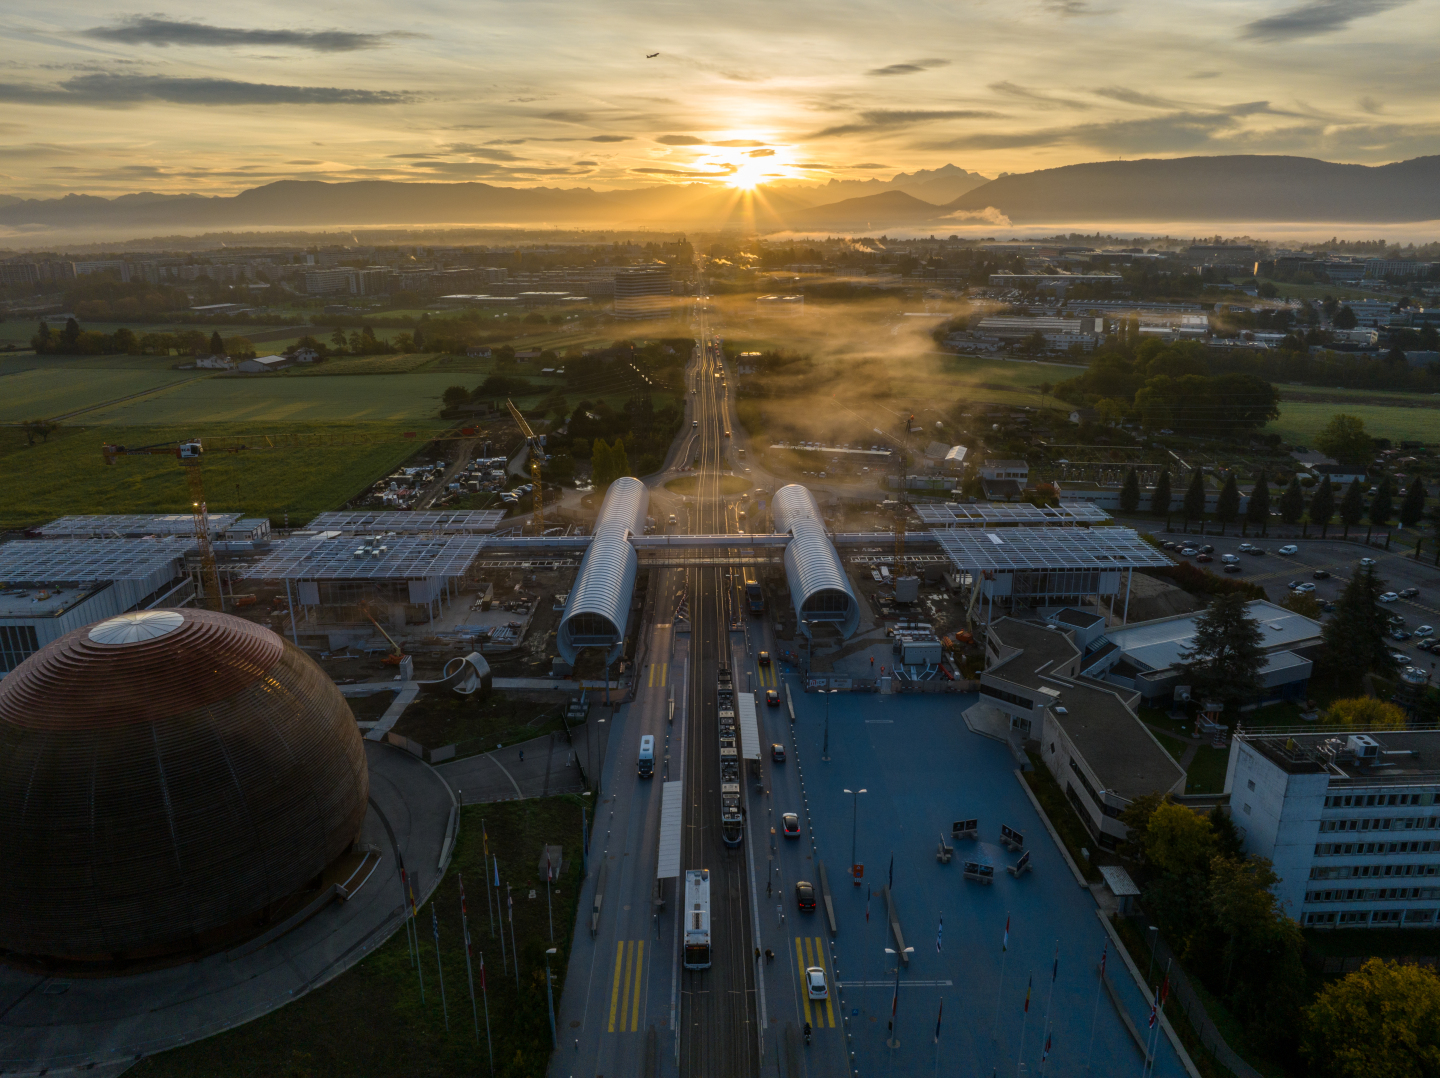
\includegraphics[width=\textwidth]{images/introduction/cern.jpg}
\caption{On the left the Globe of Science and Innovation, in the center the CERN Science Gateway designed by Renzo Piano, on the right the blue square is Place des Particules. The rest of CERN's main site develops on the right of Place des Particules \protect\cite{cern_science_gateway}}
\label{fig:science-gateway}
\end{figure}

The \acf{CERN} convention \cite{cern-convention} signed in 1953 declares that its scientific work shall be publicly shared and dedicated to peaceful advancement. At the time of writing, \ac{CERN} comprises 25 member states, with scientists from over 110 countries collaborating to decipher the fundamental structure of the universe.

Situated on the Franco-Swiss border near Geneva, \ac{CERN} hosts a chain of increasingly powerful accelerators and purpose-built detectors that operate at energies mirroring the universe's earliest moments. Major experiments such as \acs{ATLAS} \cite{atlas-experiment}, \acs{CMS} \cite{cms-experiment}, \acs{ALICE} \cite{alice-experiment}, and \acs{LHCb} \cite{lhcb-experiment} rely on the \ac{LHC} \cite{Lebrun:1284331} for their data collection. Meanwhile, projects like \acs{CLOUD} \cite{Kirkby:1310801}, \acs{ISOLDE} \cite{isolde-facility}, and NA62 \cite{Martellotti:2056863} explore complementary aspects of particle physics, expanding our knowledge on the Standard Model, which in short, is our best explanation of how the basic building blocks of matter interact \cite{standard-model}.

Beyond contributions to fundamental science, \ac{CERN} has a rich history of technological innovation, perhaps the most famous example being the creation of the World Wide Web in 1989 \cite{www-proposal}. Advances in data analysis, accelerator technology, and detector development have also impacted fields such as medical imaging, materials science, and network engineering \cite{cern-tech-impact}.

\clearpage
\section{\acs{LHC}}
\label{sec:lhc-experiments}

The \ac{LHC} \cite{Lebrun:1284331, Brüning:782076} is \ac{CERN}'s flagship accelerator and the most powerful particle collider in operation world-wide. Housed in a 27-km circular tunnel roughly 100 meters underground, it accelerates two beams of protons to 99.9999991\% the speed of light and collides them at energies up to 13.6 \ac{TeV}. Figure~\ref{fig:LHC} shows an aerial view with an overlay illustrating the geographic location of the LHC and its major experiments, giving a sense of the scale of the facility.

Particles enter the \ac{LHC} after passing through smaller accelerators (see Figure~\ref{fig:cern-complex}). A beam inside the beam pipes in the \ac{LHC} is not a continuous stream of particles, but is divided into bunches. Bunches typically contain around $10^{11}$ protons, they are spaced 25 ns apart, and collide at a rate of 40 MHz. On average, there are 43 proton-proton collisions on each bunch crossing.

\begin{figure}[htbp]
\centering
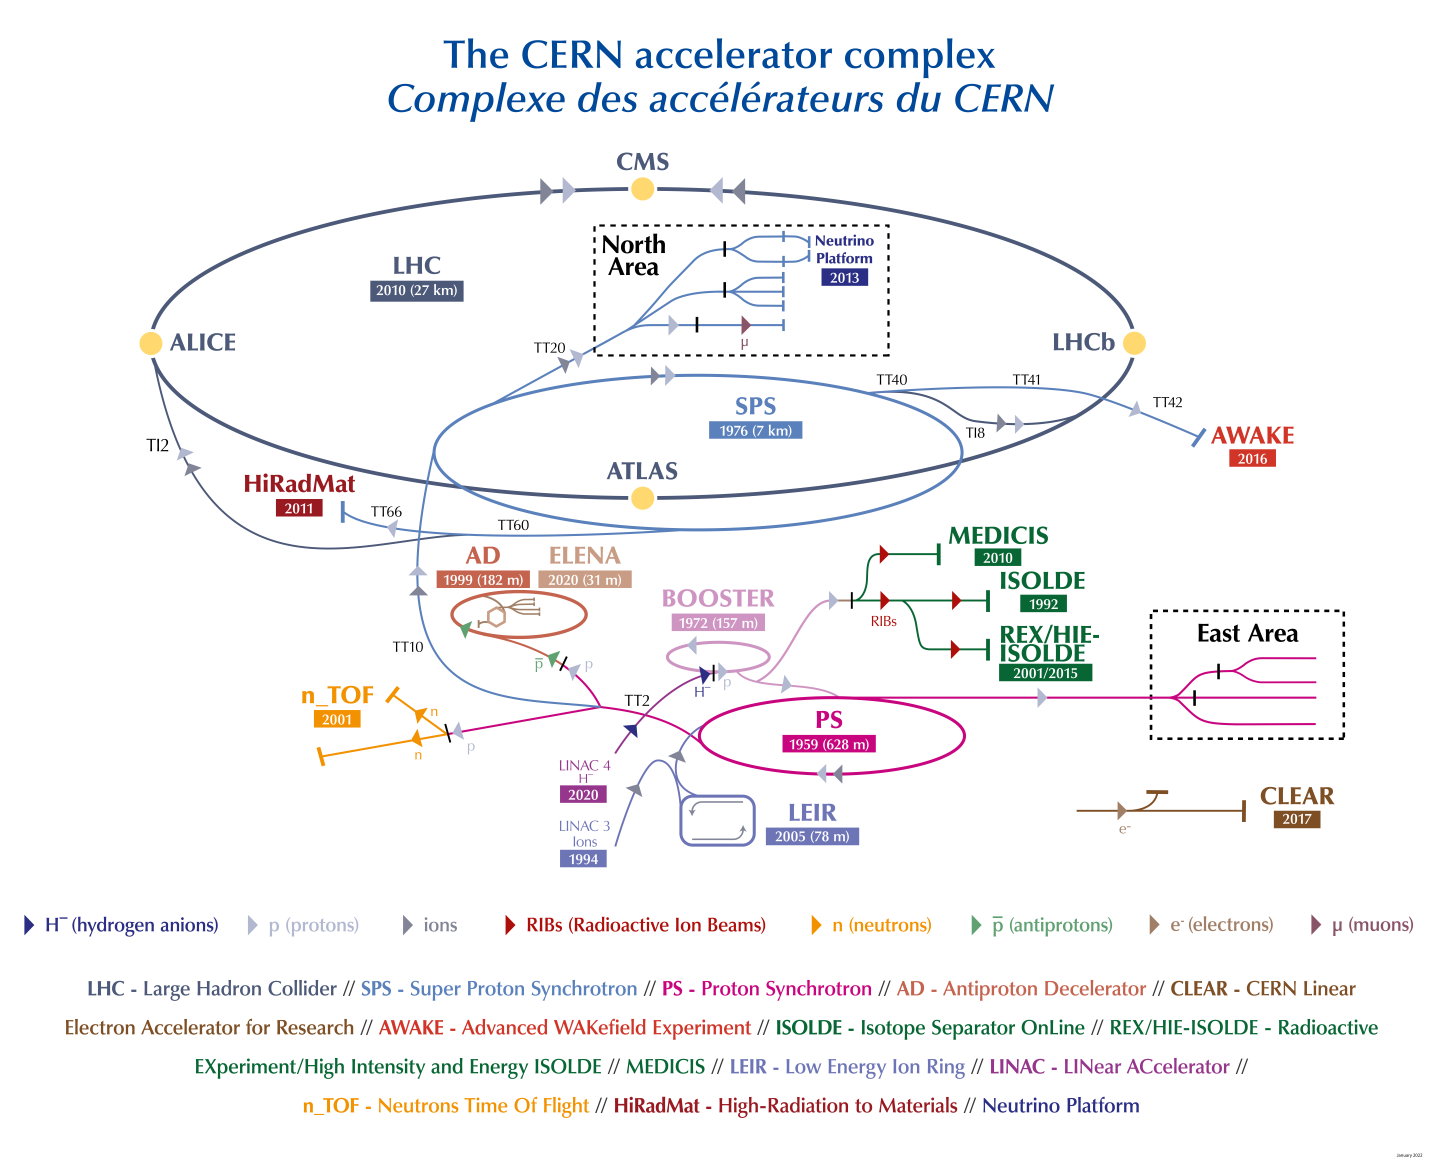
\includegraphics[width=\textwidth]{images/introduction/cern-experiments.png}
\caption[The accelerator complex at CERN]{The accelerator complex at \acs{CERN}. Several smaller accelerators boost the beam before it enters the \acs{LHC}. Primary experiments (\acs{ALICE}, \acs{ATLAS}, \acs{CMS}, \acs{LHCb}) are placed around the \acs{LHC} ring. Image source: \protect\cite{cern_accelerator_complex}}
\label{fig:cern-complex}
\end{figure}

As mentioned before, the data is gathered through four main experiments, located around the \acs{LHC} ring:
\begin{itemize}
    \item \textbf{ATLAS} \cite{atlas-experiment} and \textbf{CMS} \cite{cms-experiment}: General-purpose detectors that investigate the Higgs boson, measure quantities of the Standard Model and search for phenomena beyond it.
    \item \textbf{LHCb} \cite{lhcb-experiment}: Specializes in asymmetries between matter and antimatter, particularly in $b$-quarks. 
    \item \textbf{ALICE} \cite{alice-experiment}: Focuses on the quark-gluon plasma in heavy-ion collisions.
\end{itemize}

Regular Long Shutdowns enable maintenance and upgrades to the \acs{LHC} and its experiments. These planned intervals improve performance and add new features, ensuring the facility meets new scientific objectives, including the transition toward the High-Luminosity \acs{LHC} phase.

\begin{figure}[H]
\centering
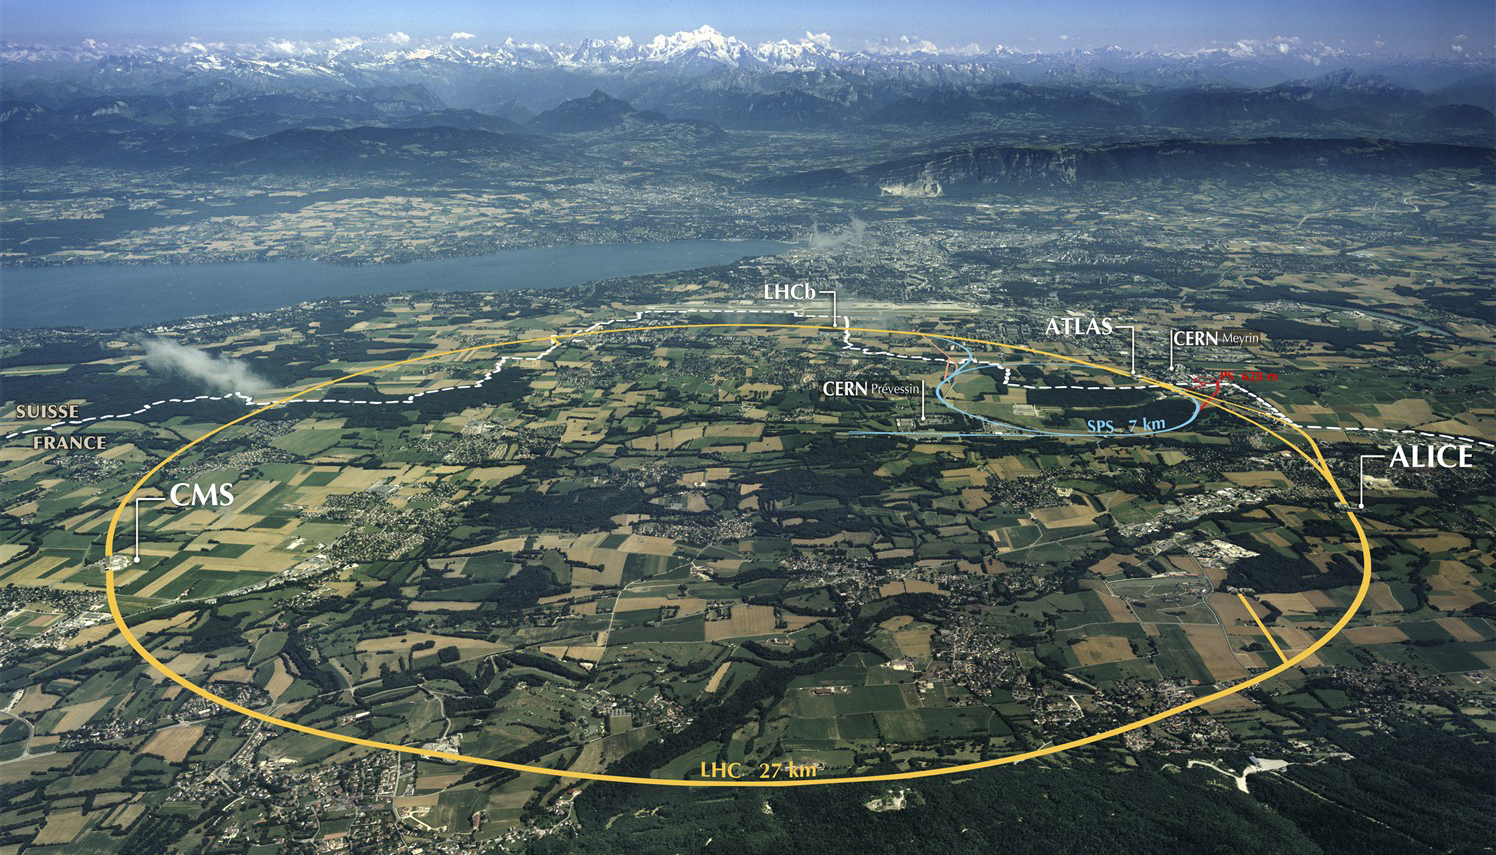
\includegraphics[width=\textwidth]{images/introduction/LHC_map.jpg}
\caption{An approximate overlay of the \acs{LHC}'s underground tunnel. \protect\cite{lhc_tunnel_map}}
\label{fig:LHC}
\end{figure}

\subsection{The High-Luminosity \acs{LHC} Era}

\ac{CERN} is preparing for \acf{LS3}, after which the \acs{HL-LHC} era begins around June 2030, as shown in Figure~\ref{fig:LHC-schedule} which displays the schedule up to the year 2041. The \acf{HL-LHC} aims to increase luminosity by an order of magnitude over the original design, enabling data collection at rates of up to 200 simultaneous proton-proton collisions per bunch crossing. This high collision density compels substantial upgrades in \acs{ATLAS} detectors and online systems.

\begin{figure}[H]
\centering
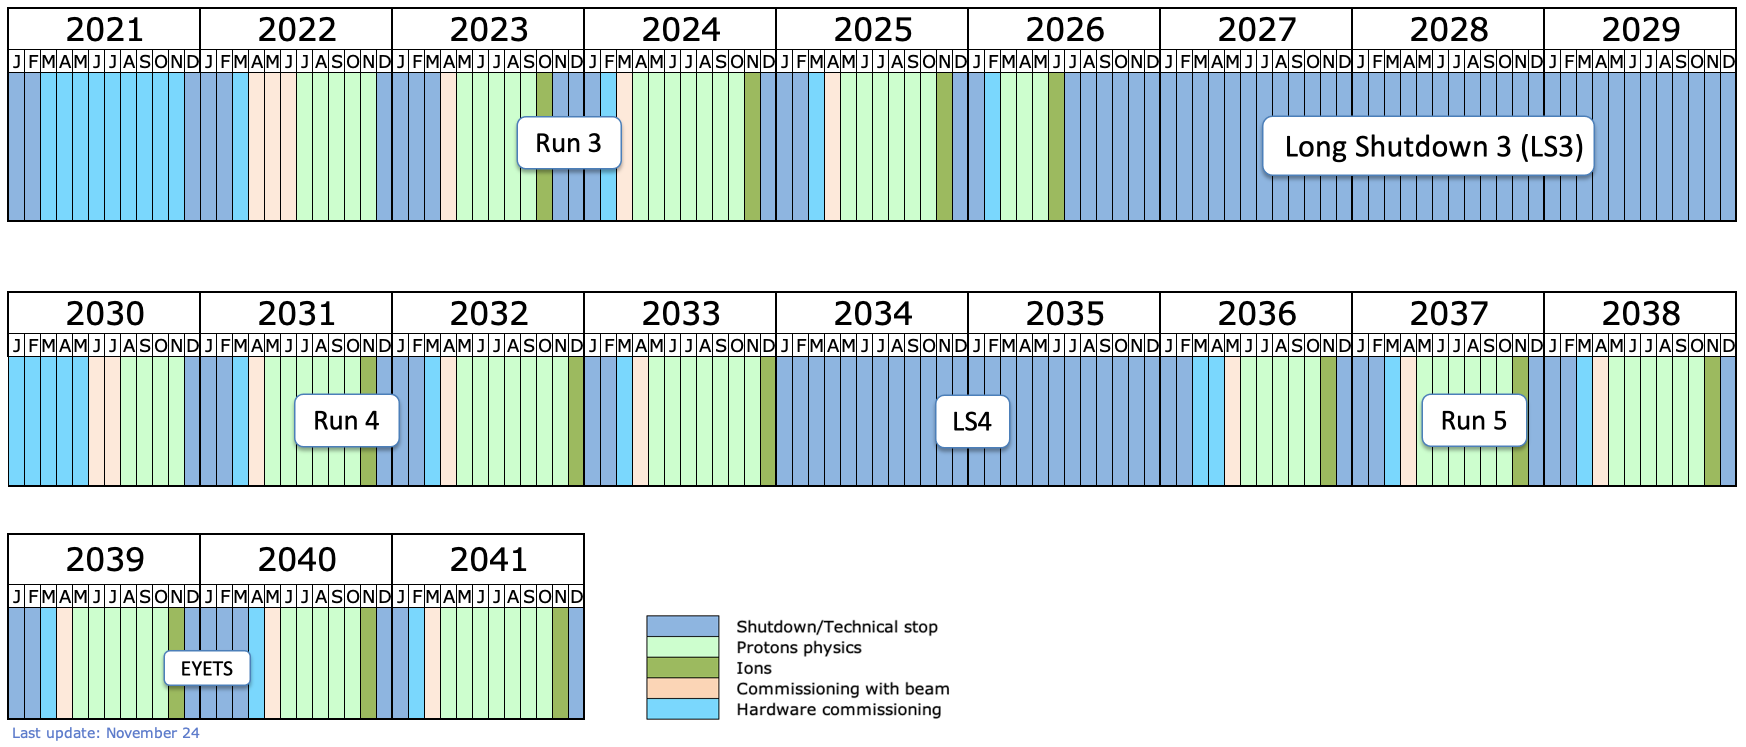
\includegraphics[width=\textwidth]{images/introduction/LHC-schedule.png}
\caption[Upgrade schedule for the LHC]{Upgrade schedule for the LHC. LS3 marks the start of HL-LHC conditions. \protect\cite{lhc_upgrade_schedule}}
\label{fig:LHC-schedule}
\end{figure}

\clearpage
\section{ATLAS Experiment}

The \acs{ATLAS} detector \cite{atlas-experiment}, central to this thesis, is the largest general-purpose experiment at the \acs{LHC}. Comparable in size to a multistory building (44 m in length and 25 m in diameter), \acs{ATLAS} features multiple layers of specialized subsystems (detectors), each engineered to measure distinct particle properties. Key scientific goals include precision studies of the Higgs boson (discovered in 2012 \cite{atlas-higgs-discovery}) and searches for supersymmetric particles.

\begin{figure}[H]
\centering
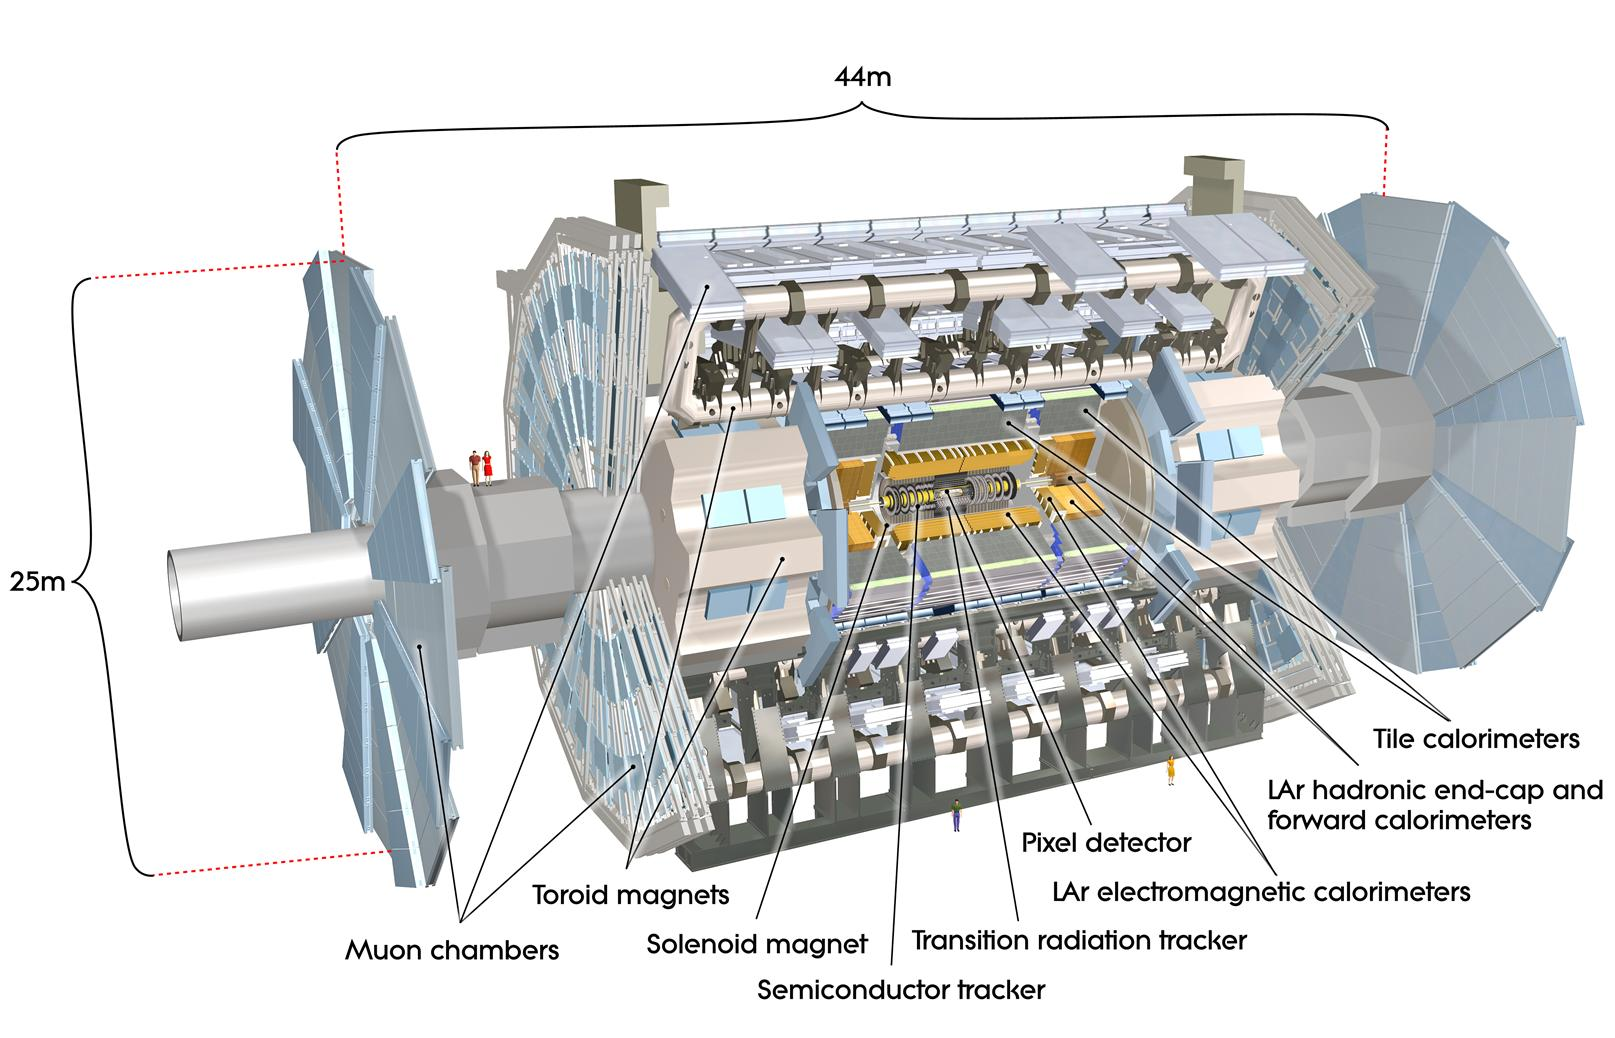
\includegraphics[width=\textwidth]{images/introduction/atlas-model.jpg}
\caption[Schematic of the ATLAS detector]{Schematic of the \acs{ATLAS} detector. Two primary magnet systems bend charged particle trajectories. The detectors measure particle energy and momentum. Image source: \acs{ATLAS} experiment. \protect\cite{atlas-experiment}}
\label{fig:atlas-model}
\end{figure}

Operated by a global collaboration of over 5,000 scientists, \acs{ATLAS} sits about 100 meters below ground. A separate service cavern (USA15) houses cooling and readout electronics, which are connected to the detectors via optical fibers. Because of intense magnetic fields and radiation, the \acs{lpGBT} \acs{ASIC} \cite{lpgbt} has been developed to allow multipurpose high speed bidirectional optical links between the detectors and readout system.

\begin{figure}[H]
\centering
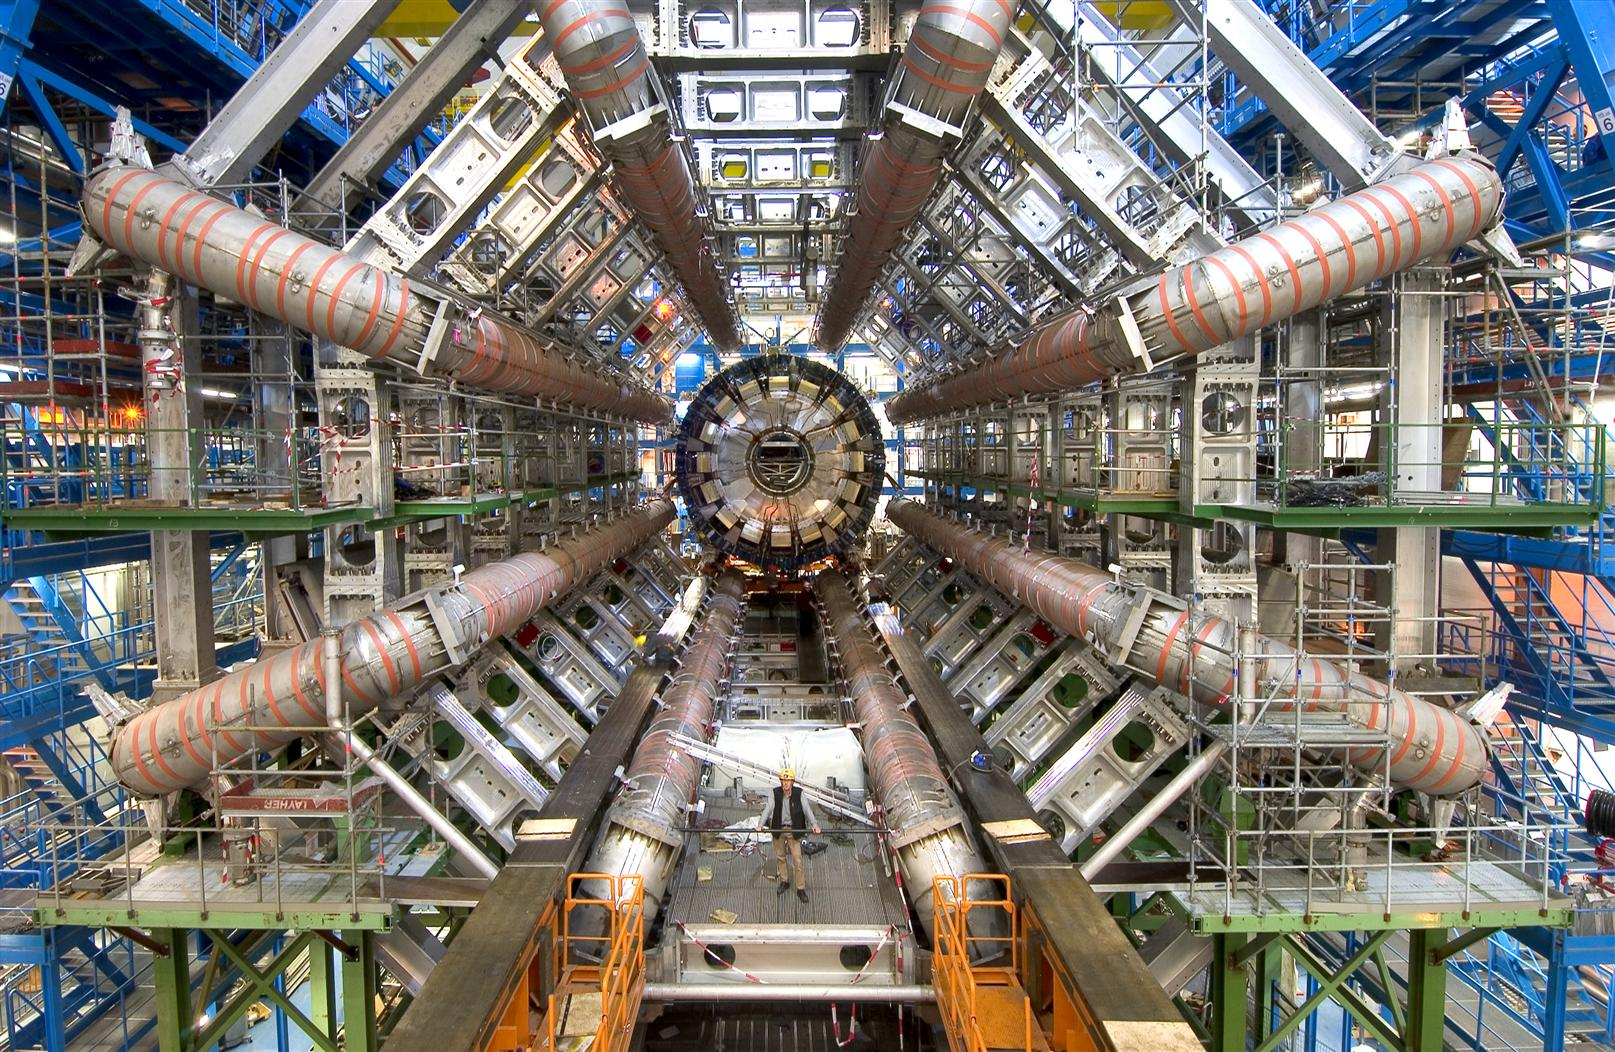
\includegraphics[width=\textwidth]{images/introduction/atlas.jpg}
\caption{A view of the ATLAS detector installation. \protect\cite{atlas-experiment}}
\label{fig:atlas}
\end{figure}

\subsubsection{\acs{ATLAS} Phase II}

The \acs{ATLAS} Phase II upgrade \cite{Affolder:2799535} adapts the experiment to make use of the \acs{HL-LHC}'s higher luminosity. 
More precisely, the \acs{HL-LHC} will deliver 10 times more data compared to the previous run.  To meet the challenges \acs{ATLAS} will include a new \acf{HGTD} \cite{hgtd-phase2-upgrade} for a better time measurement, a new all-silicon \acf{ITk} \cite{atlas-itk-pixel-detector}, and a new \acs{T-DAQ} system capable of handling data arriving at 1 MHz.

\clearpage
\section{\acf{T-DAQ}}

As the name suggests, the \acs{ATLAS} \acf{T-DAQ} system is composed of a Trigger and a \acf{DAQ} system. Figure~\ref{fig:tdaq} provides a high level description of the \acs{T-DAQ} architecture showing the Detectors layer and the Event Filter layer tt the bottom. A more in-depth description of each architectural component is presented below.

\begin{figure}[htbp]
\centering
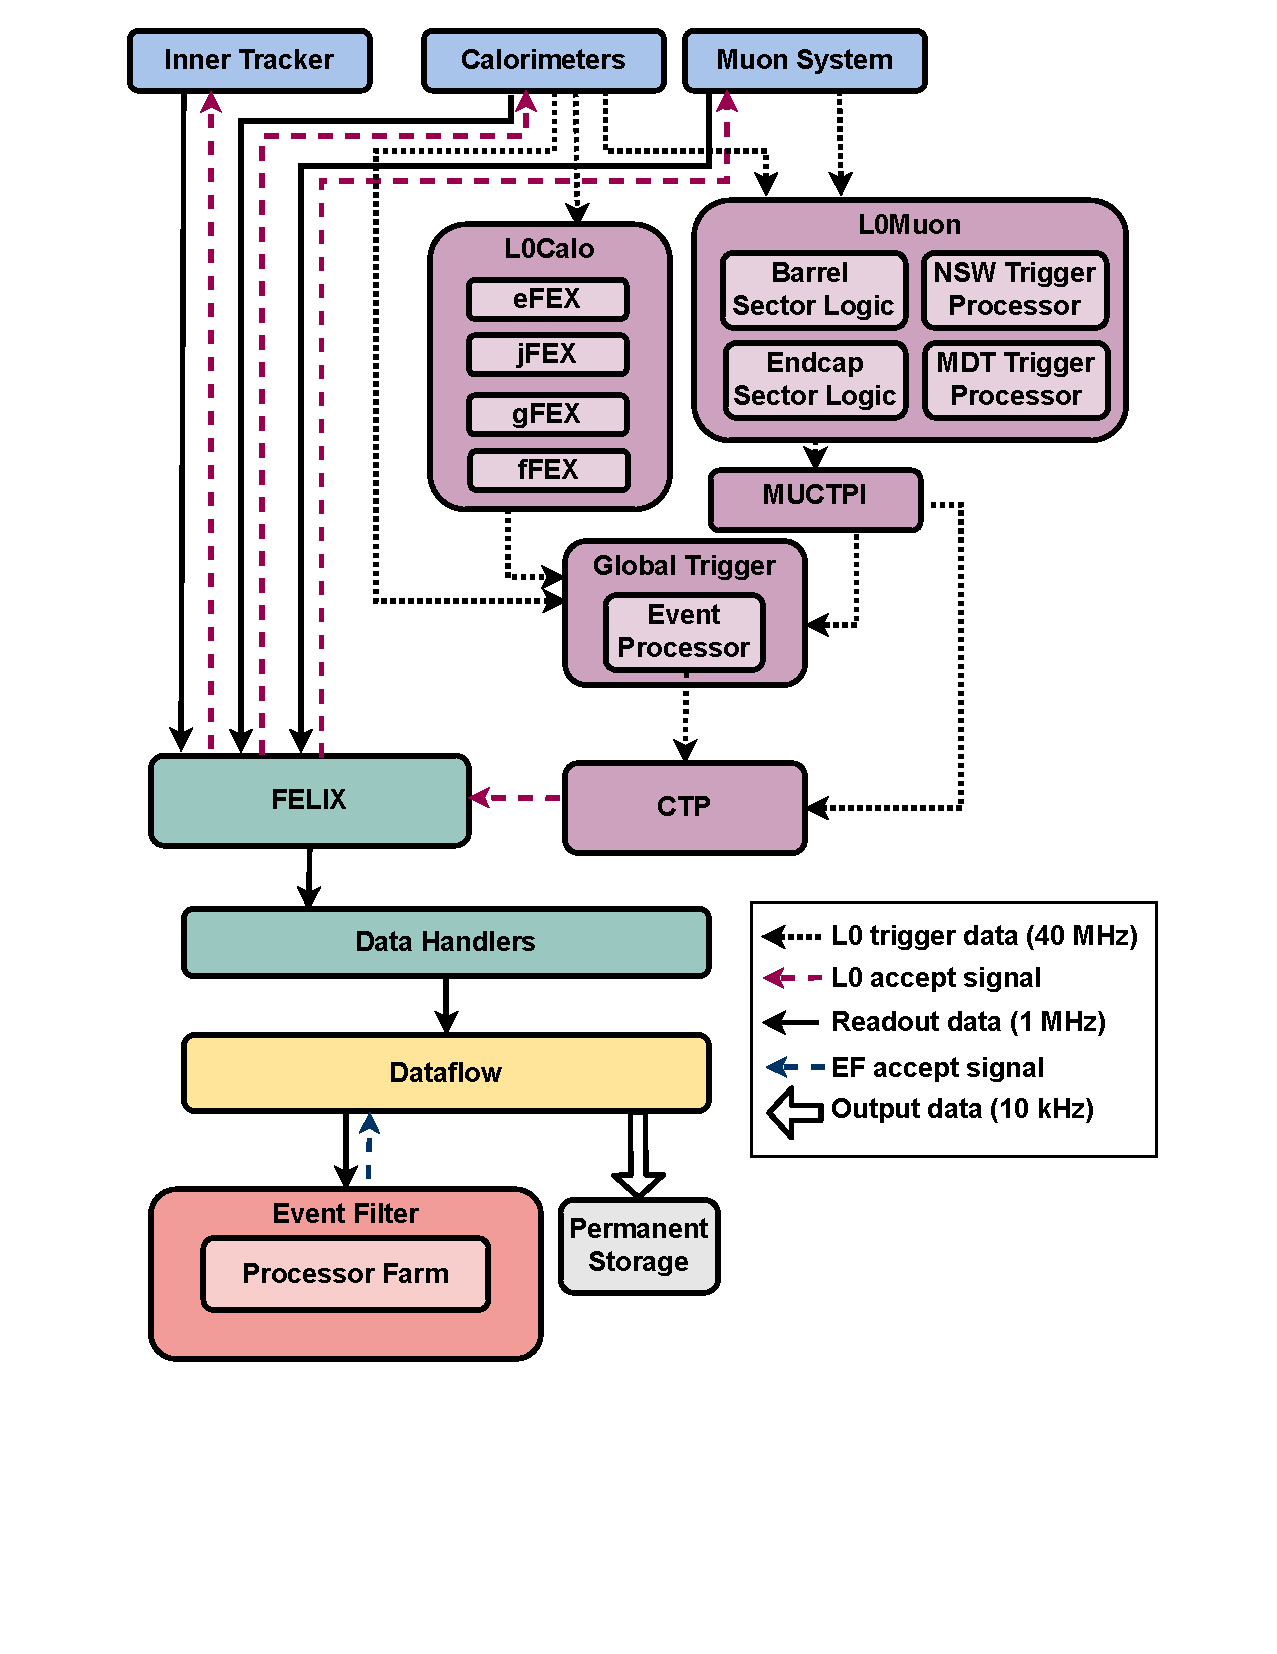
\includegraphics[width=0.68\textwidth]{images/introduction/Baseline_TDAQ_Phase-II_Architecture.pdf}
\caption[Overview of the T-DAQ architecture]{An overview of the \acs{T-DAQ} architecture is shown. The three main layers are color-coded: the Level-0 Trigger in pink, the DAQ subsystem (comprising the Readout and Dataflow subsystems) in green and yellow, and the Event Filter at the bottom in red. The detectors, shown in blue, are not part of the T-DAQ infrastructure but are included to provide context on how T-DAQ interfaces with other components of the \acs{ATLAS} experiment. Image source: \protect\cite{tdaq}}
\label{fig:tdaq}
\end{figure}

\subsection{Trigger}

\begin{definition}
\label{def:event}
An event captures the hits generated by a collision in a bunch crossing observed by detectors.
\end{definition}

This can reach data volumes of roughly 60 TB/s. The duty of triggers is to filter out non-interesting events.

\begin{definition}
\label{def:trigger}
A trigger is a hard- or software-based filter that issues \emph{ACCEPT} or \emph{REJECT} decisions for each event.
\end{definition}

Triggers may examine particle counts, reconstructed energy, momenta, or other indicators of interesting physics.

The Trigger layer that forms a first-level hardware based trigger includes \cite{tdaq} \acs{L0Calo}, \acs{L0Muon} (\acs{L0} stands for Level 0, which is a term used for components detached from the main detector that perform a first filtering of the events), the Global Trigger, and the Central Trigger Subsystem (\acs{CTP}). Essentially, \acs{L0Calo} filters for the energies and positions of charged and neutral particles, \acs{L0Muon} is used to filter for muons, and the \acs{MUCTPI}'s task is to interface \acs{L0Muon} with \acs{CTP}. The Global Trigger \cite{tdaq} uses full-granularity calorimeter information to perform offline-like algorithms, refines the trigger objects calculated by \acs{L0Calo} and \acs{L0Muon}, calculates event-level quantities, and executes topological algorithms. The \acs{CTP} \cite{tdaq} forms triggers based on combinations of inputs or conditions received from the Global Trigger and other sources; it applies pre-scale factors and introduces deadtime when necessary to avoid saturation in the front-end and readout systems. Ultimately, it makes the final decision on whether the event is accepted, driving the \acs{TTC} network to start the readout process of the detectors.

\subsection{\acs{DAQ} - Readout and Dataflow}

\begin{definition}
\label{def:daq}
A data acquisition system \acs{DAQ} aggregates detector data, relays trigger outcomes, and writes all accepted events to permanent storage.
\end{definition}

In the Readout layer is shown that the Data Handler can receive data only from the \acs{FELIX} card \cite{tdaq}, also the \acs{FELIX} card is directly linked to the Detectors via an optical interface, other than the \acs{L0} Triggers. The \acs{FELIX} card receives data fragments from the detectors, sends them to the Data Handlers that re-organizes those fragments for detector-specific operations that will be performed by the Dataflow.

The Dataflow system \cite{tdaq} as shown in the previous Figure~\ref{fig:tdaq} includes all components needed to aggregate the data fragments towards a full event-building, to buffer the events for the software trigger (Event Filter) and send the selected event to permanent storage.

\subsection{Event Filter}

The Event Filter system \cite{tdaq} consists of a CPU-based processing farm. The EF system runs more elaborate algorithms that take the data from the entire detector to reduce the trigger rate by another order of magnitude to get it down to the final output rate of 10 KHz. Events will be rejected as early as possible during their processing. The Event Filter decisions will be communicated to the Dataflow, which will then transfer the accepted events to permanent storage.

\clearpage
\section{\acs{FELIX}}

Within the \acs{T-DAQ} architecture, \acs{FELIX} offers an interface between detector front-end electronics and downstream data processing. It is designed to handle the high data rates projected for the forthcoming HL-LHC phase and allows for a flexible, high-throughput readout system.

\subsubsection{\acs{FELIX} in Phase II}

\begin{figure}[H]
\centering
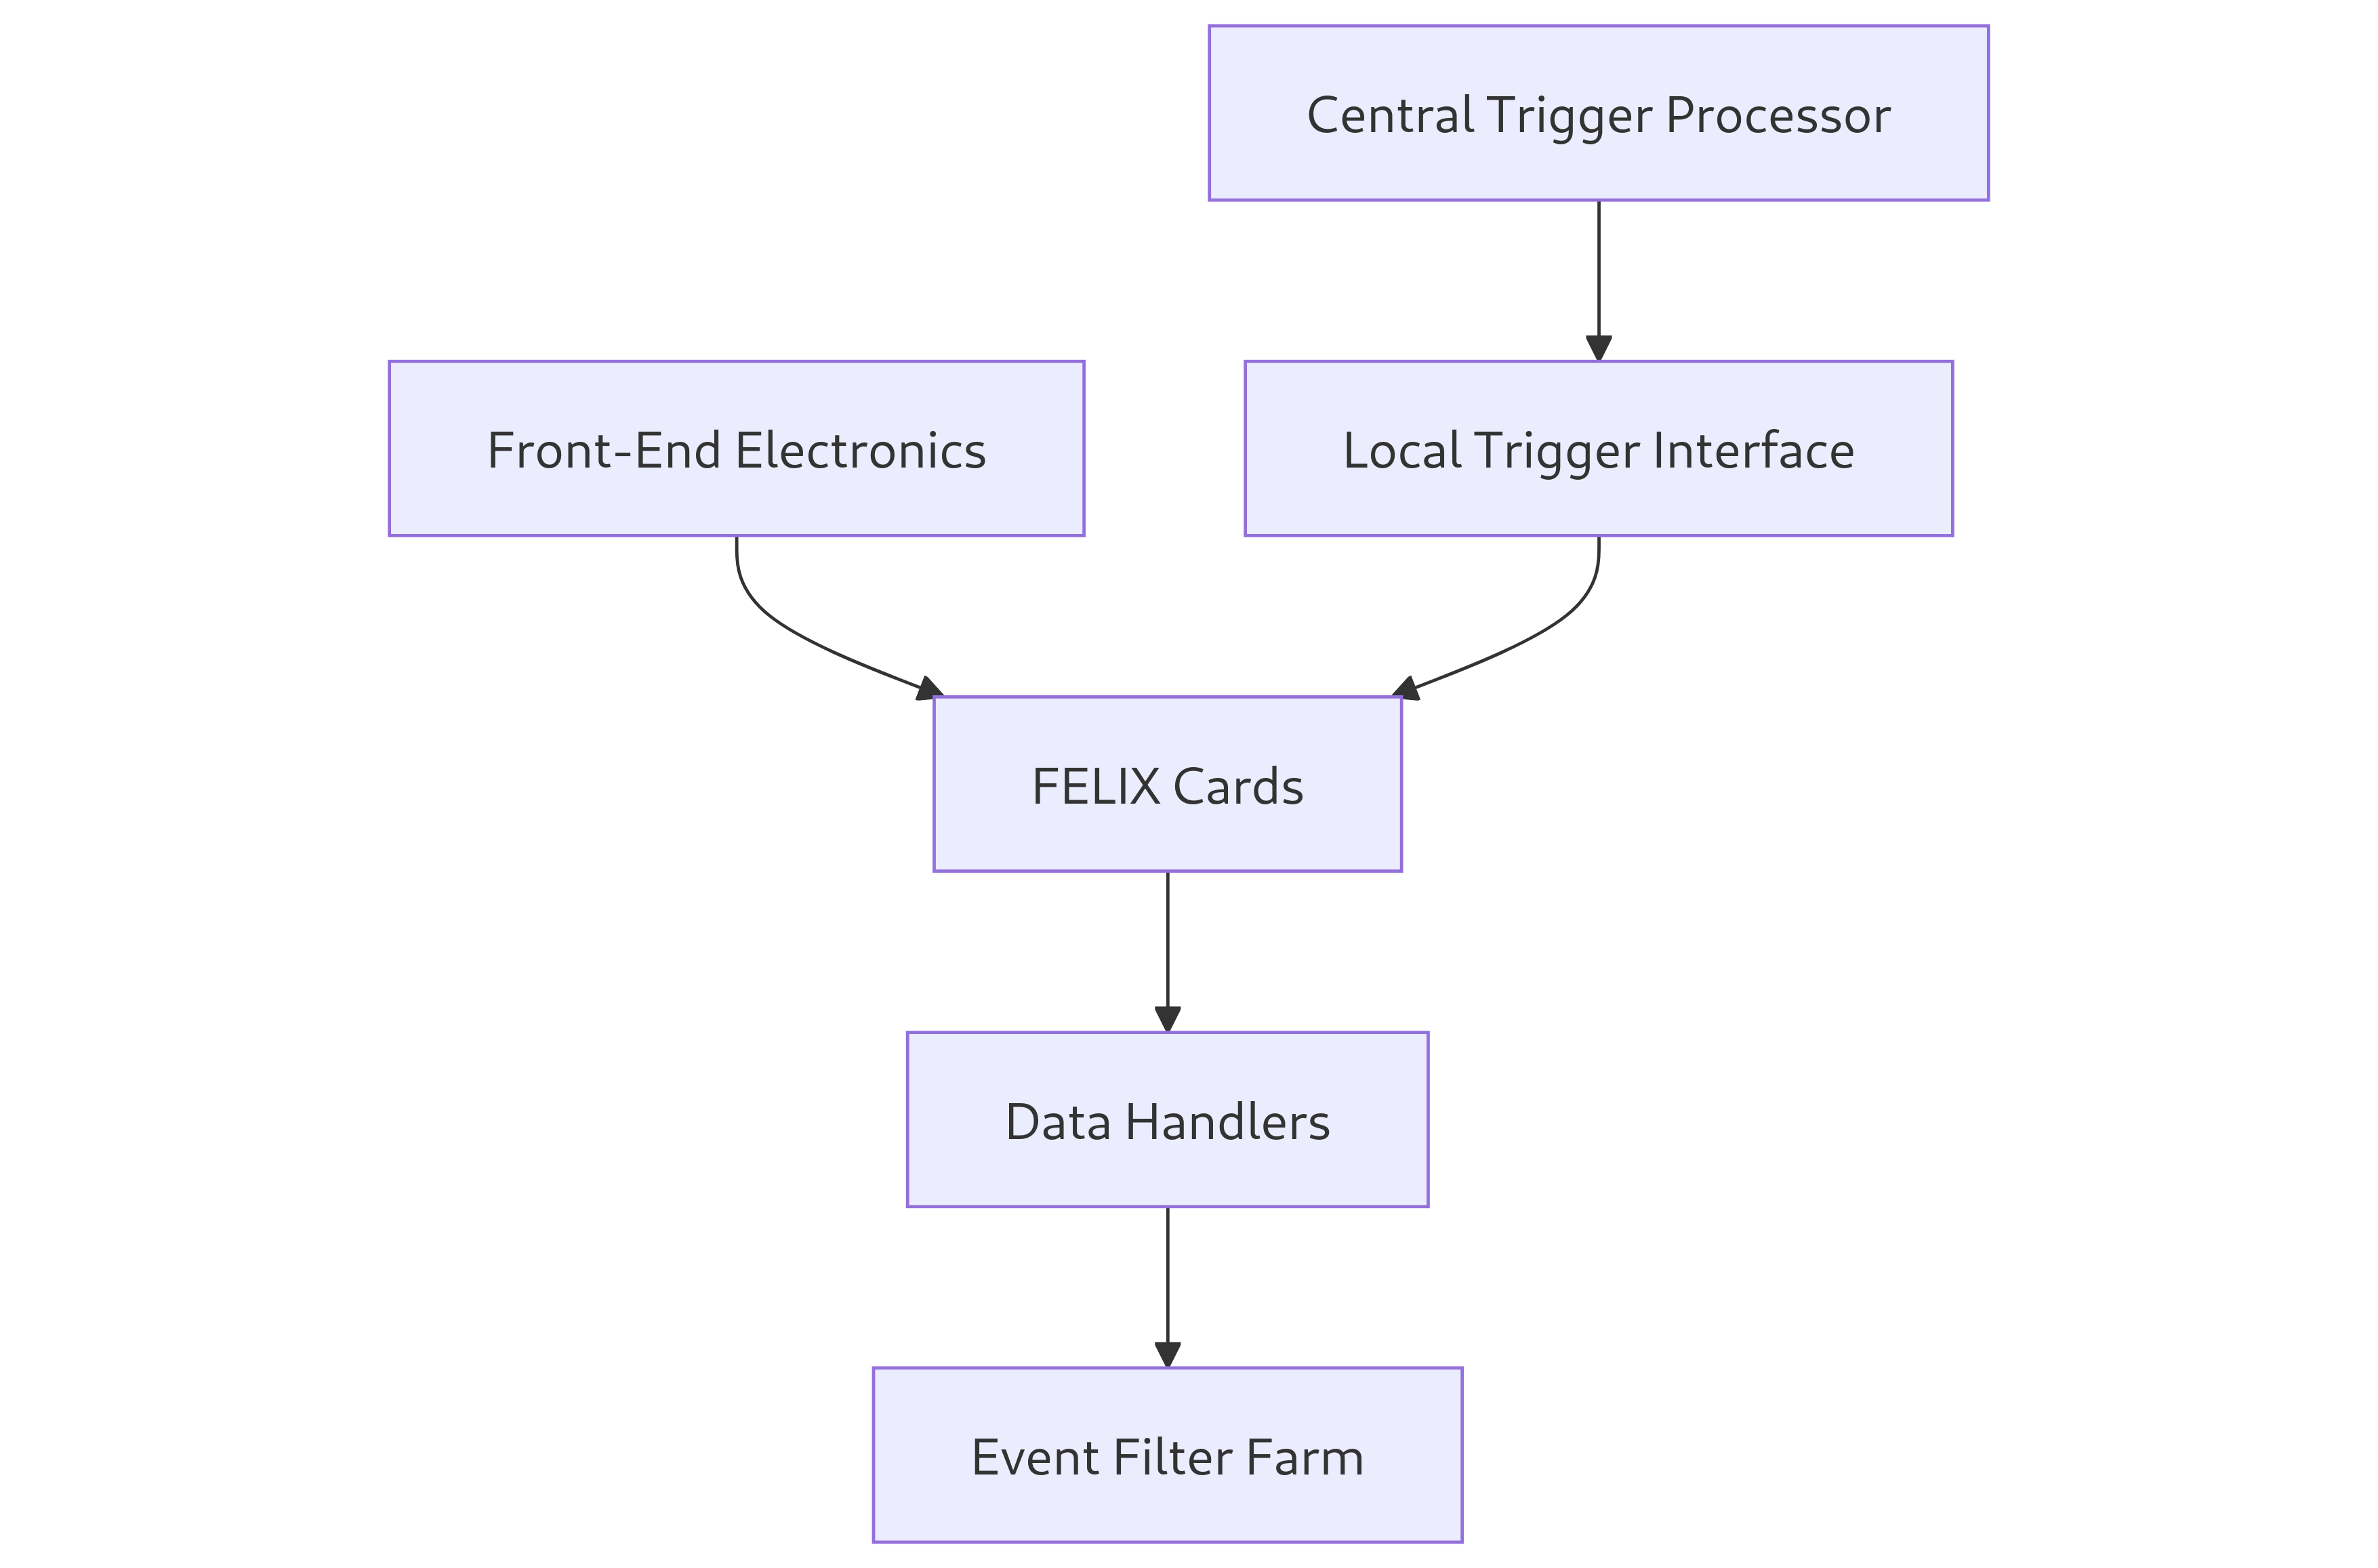
\includegraphics[width=\textwidth]{images/introduction/felix-block-diagram.png}
\caption[Block diagram of the Readout system]{Block diagram of the Readout system, focusing on the FELIX part. It is connected to Front-End Electronics, Data Handler, Event Filter Farm, and \acf{LTI}.}
\label{fig:felix-block-diagram}
\end{figure}

\acs{FELIX} radout system will be linking upgraded front-end electronics to commercial servers through \acs{FPGA}-based \acs{PCIe} cards. It will be translating detector-specific protocols into standard network packets, allowing the detectors to communicate with the Data Handlers.\\
This last part is the main answer of why \acs{FELIX} is needed in the \acs{T-DAQ} architecture. On-detector electronics must be radiation tolerant. For this purpose at \acs{CERN} have been developed custom electronics, like \acl{lpGBT} \cite{lpgbt} that uses its own protocol, but the rest of the underlying architecture uses normal network protocols since they are shielded from radiations; \acs{FELIX} is in between the two layers allowing them to communicate.\\
The new \acs{FELIX} system can handle event rates in excess of 1 MHz and data streams beyond 5~TB/s, and allows for:
\begin{itemize}
    \item \textbf{Scalability}: Commodity server hardware reduces the cost and simplifies maintenance compared to purely custom designs.
    \item \textbf{System Flexibility}: Uniform support for various upgraded detector systems, including the new \acs{ITk} detector and \acs{HGTD}.
    \item \textbf{Low-Latency}: Low latency and minimal data loss are important to reach the \acs{HL-LHC} objectives.
\end{itemize}

\subsubsection{Scale and Implementation of the \acs{FELIX} System}

The \acs{ATLAS} Phase-II Readout System is responsible for collecting data from all detector subsystems and preparing it for processing by the Dataflow and Event Filter layers. It is made up of two main parts: \acs{FELIX} and the \acf{DH}.

\paragraph{FELIX.}
\acf{FELIX} acts as the bridge between the detector front-end electronics and the computing infrastructure. It connects directly to the detectors through high-speed optical links and converts their data into a format that can be handled by standard network equipment.

Each \acs{FELIX} server hosts two custom \acs{PCIe} cards (FLX-155). The FLX-155 will be presented later in more detail (Section~\ref{subsec:FLX-155}). The card is designed around AMD Versal \acs{FPGA}s. These cards support up to 48 optical links each, and the number of active links depends on the specific detector and the bandwidth needed. For example, the \acs{ITk} Strips detector uses cards with up to 336 logical links per card.

Once the data is received, \acs{FELIX} uses a high-speed 200~Gb/s network interface to send it to the next stage: the Data Handler servers.

\paragraph{Data Handlers.}
The Data Handlers are a set of dedicated servers that receive data from \acs{FELIX} and perform two main tasks. First, they rebuild complete detector "fragments" by combining data that belongs to the same event. Then, they pass those fragments to the Dataflow system for further processing.

Depending on the detector, the \acs{DH} may work in two different modes. For some detectors—like \acs{ITk}, \acs{HGTD}, and New Small Wheel, the data arrives in small pieces from many sources, and the \acs{DH} must perform "fragment building." This requires more computing power, as it involves grouping, formatting, and validating the data. For other detectors that already send pre-formatted fragments, the \acs{DH} simply acts as a relay.

\paragraph{Infrastructure and Constraints.}
The entire Readout System will be installed in the USA15 underground counting room, which has strict limits on available space and cooling. There are 36 server racks available, each with a 15~kW power budget.

In total, the system will include:
\begin{itemize}
    \item 783 \acs{FELIX} cards (including spares),
    \item 371 \acs{FELIX} servers (2 cards per server),
    \item 701 Data Handler servers.
\end{itemize}

Together, these components consume around 495~kW of power, filling all available racks.


